\documentclass[tikz,border=6pt]{standalone}
\usepackage{amsmath,amssymb}
\begin{document}
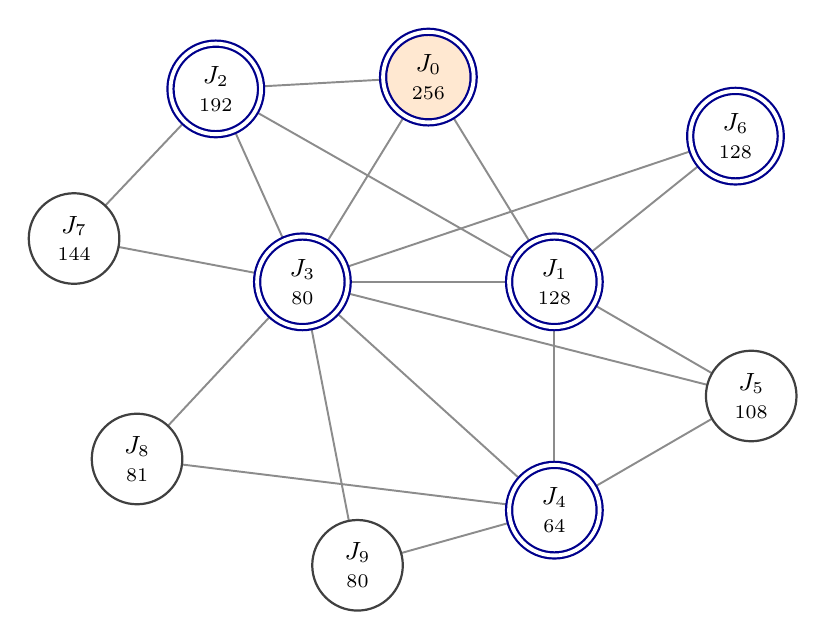
\begin{tikzpicture}[
  v/.style={circle,draw=black!75,fill=white,thick,minimum size=11.5mm,inner sep=0pt,align=center,font=\small},
  u/.style={v,double=white,double distance=1.4pt,draw=blue!55!black},
  best/.style={u,fill=orange!18},
  e/.style={draw=black!45,line width=0.7pt}]
  % two hubs, J_3 and J_1, and the other classes around them
  \coordinate (p3) at (-1.6,0);
  \coordinate (p1) at (1.6,0);
  \coordinate (p0) at (0,2.6);
  \coordinate (p2) at (-2.7,2.45);
  \coordinate (p7) at (-4.5,0.55);
  \coordinate (p8) at (-3.7,-2.25);
  \coordinate (p9) at (-0.9,-3.6);
  \coordinate (p4) at (1.6,-2.9);
  \coordinate (p5) at (4.1,-1.45);
  \coordinate (p6) at (3.9,1.85);
  % edges between different classes (Table 5.2)
  \foreach \k in {0,1,2,4,5,6,7,8,9} \draw[e] (p3)--(p\k);
  \foreach \k in {0,2,4,5,6} \draw[e] (p1)--(p\k);
  \draw[e] (p0)--(p2) (p2)--(p7) (p4)--(p5) (p4)--(p8) (p4)--(p9);
  % nodes
  \node[u]    at (p3) {$J_3$\\[-1pt]\scriptsize $80$};
  \node[u]    at (p1) {$J_1$\\[-1pt]\scriptsize $128$};
  \node[best] at (p0) {$J_0$\\[-1pt]\scriptsize $256$};
  \node[u]    at (p2) {$J_2$\\[-1pt]\scriptsize $192$};
  \node[v]    at (p7) {$J_7$\\[-1pt]\scriptsize $144$};
  \node[v]    at (p8) {$J_8$\\[-1pt]\scriptsize $81$};
  \node[v]    at (p9) {$J_9$\\[-1pt]\scriptsize $80$};
  \node[u]    at (p4) {$J_4$\\[-1pt]\scriptsize $64$};
  \node[v]    at (p5) {$J_5$\\[-1pt]\scriptsize $108$};
  \node[u]    at (p6) {$J_6$\\[-1pt]\scriptsize $128$};
\end{tikzpicture}
\end{document}
